\labsection{3}{Search Engineering: Package, Tests, CLI, and Benchmark}{sec:lab03-search-code}

\begin{labproject}{Turn Labs 1--2 into a reproducible Python toolkit}
\textbf{Read first.} Chapter~\ref{ch:searchpatterns}.\\
\textbf{Goal.} Standardise five algorithms, verify them with dataset-free tests, expose a command-line interface, and benchmark ten route queries.\\
\textbf{Scenario.} Convert notebook logic into reusable, testable software.\\
\textbf{Data.} The OpenFlights files and \texttt{all\_experiments/utils/search\_queries.csv}; unit tests use hand-made graphs.\\
\textbf{Notebook.} \texttt{all\_experiments/lab03\_search\_engineering\_worked.ipynb}; implementation and tests are in \texttt{all\_experiments/utils/}.\\
\textbf{Hand in.} The executed notebook, the \texttt{results/lab03/} folder and a short conclusion, as listed in the checklist at the end of this sheet.
\end{labproject}

\begin{labmode}
\begin{enumerate}
  \item Activate your course environment.
  \item From \texttt{all\_experiments/}, run the tests and one route search in a terminal. These two commands should work before you open the notebook.
  \item Start Jupyter from the same folder, open the notebook, and choose \textbf{Restart Kernel and Run All Cells}. Everything runs in a few seconds.
\end{enumerate}
\begin{lstlisting}[style=utpterminal]
cd all_experiments
python -m pytest utils -q
python -m utils --algorithm astar --start KUL --goal KEF
jupyter lab
\end{lstlisting}
Prefer a plain script? From the course folder, \texttt{python all\_experiments/lab03\_search\_engineering\_worked.py} runs the same code and writes the same evidence.
\end{labmode}

\courselabflow{Define API}{Test tiny graphs}{Run CLI}{Benchmark routes}


\labroutine

\begin{yourturn}
\textbf{Warm-up on paper.} The notebook's tiny graph is below. Before running anything, write down the path and cost you expect from each of BFS, DFS, UCS, GBFS and A$^\star$. The heuristic is $h(S)=5$, $h(A)=4$, $h(B)=1$, $h(G)=0$.
\begin{lstlisting}[style=utppython]
toy = {"S": [("A", 2.0), ("B", 5.0)], "A": [("G", 5.0)], "B": [("G", 1.0)], "G": []}
\end{lstlisting}
\end{yourturn}

\textbf{Setup.} Run the imports and path setup first, and keep this kernel state for the later questions. In the script version the first seven lines also set the working directory.
\lstinputlisting[style=utppython,firstline=1,lastline=7]{all_experiments/lab03_search_engineering_worked.py}
\lstinputlisting[style=utppython,firstline=8,lastline=23]{all_experiments/lab03_search_engineering_worked.py}

\textbf{Read the shared search engine.} Labs~1 and~2 used this module without looking inside. Read it now, in five parts, before running the engineering checks. It lives at \texttt{all\_experiments/utils/core.py}, and the package initialiser exposes these functions to every notebook.

\noindent\textbf{Result record and path reconstruction.}
\lstinputlisting[style=utppython,firstline=1,lastline=42]{all_experiments/utils/core.py}
\noindent\textbf{Cost accounting and BFS.}
\lstinputlisting[style=utppython,firstline=43,lastline=74]{all_experiments/utils/core.py}
\noindent\textbf{DFS and the priority-frontier interface.}
\lstinputlisting[style=utppython,firstline=75,lastline=106]{all_experiments/utils/core.py}
\noindent\textbf{Priority search, stale entries and termination.}
\lstinputlisting[style=utppython,firstline=107,lastline=135]{all_experiments/utils/core.py}
\noindent\textbf{UCS, greedy and A$^\star$ entry points.}
\lstinputlisting[style=utppython,firstline=136,lastline=148]{all_experiments/utils/core.py}

\begin{labquestion}{1}{Standardise the interface}
Every algorithm must return the same fields. Show the fields of \texttt{SearchResult}, then run all five algorithms on the small hand-made graph and display the results as one table.
\end{labquestion}
\begin{labanswer}
\courselabtrace{Keep responsibilities separate}{Loader}{CSV rows become a weighted graph}{Search}{Graph and endpoints become SearchResult}{Reporter}{Result becomes a table or route plot}

Use this fixture before the airline benchmark. A hop-minimising algorithm can choose either two-hop route according to its neighbour order, because it does not look at their weights.
\courselabtrace{Trace the actual search-engineering fixture}{1. Input / state}{toy has S to A cost 2, S to B cost 5, A to G cost 5, and B to G cost 1.}{2. Operation}{Routes S-A-G and S-B-G both have two hops; their costs are 7 and 6.}{3. Check}{UCS selects cost 6. With the supplied consistent h, A-star must also return cost 6.}


\lstinputlisting[style=utppython,firstline=25,lastline=39]{all_experiments/lab03_search_engineering_worked.py}
\begin{refoutput}
\begin{lstlisting}[style=utpterminal]
SearchResult fields: ['found', 'path', 'hops', 'path_cost_km', 'expanded', 'max_frontier', 'runtime_ms']
      path          hops  cost  expanded  max_frontier
BFS   S -> A -> G      2   7.0         3             2
DFS   S -> A -> G      2   7.0         2             2
UCS   S -> B -> G      2   6.0         3             2
GBFS  S -> B -> G      2   6.0         2             2
A*    S -> B -> G      2   6.0         3             2
\end{lstlisting}
\end{refoutput}

\textbf{What it means.} All five functions return a \texttt{SearchResult} with identical fields, so one loop can benchmark them. BFS and DFS return the two-edge route through A at cost 7, while UCS and A$^\star$ return the cheaper route through B at cost 6. GBFS also picks B, because $h(B) < h(A)$.
\end{labanswer}

\begin{labquestion}{2}{Separate responsibilities}
Search logic, data loading, plotting and the command line must live in separate modules. List the package's modules with their one-line purpose, and the names it exports.
\end{labquestion}
\begin{labanswer}
\lstinputlisting[style=utppython,firstline=41,lastline=45]{all_experiments/lab03_search_engineering_worked.py}
\begin{refoutput}
\begin{lstlisting}[style=utpterminal]
__init__.py      Helper code for the AI course notebooks.
__main__.py      Command-line route search (Lab 3).
core.py          Graph-search algorithms shared by Labs 1-3: BFS, DFS, UCS, GBFS and A*.
openflights.py   Load the OpenFlights airport and route files into a weighted graph.
plotting.py      Plot airport routes on longitude/latitude axes (Labs 1-3).
test_search.py   Unit tests for utils.core on tiny hand-made graphs (no dataset needed).

Exported names: SearchResult, astar, best_first, bfs, dfs, gbfs, ucs, haversine_km, load_openflights, route_is_valid, plot_route_paths
\end{lstlisting}
\end{refoutput}

\textbf{What it means.} \texttt{core.py} holds the five algorithms and knows nothing about airports; \texttt{openflights.py} cleans the CSV files and computes distances; \texttt{plotting.py} draws routes; \texttt{\_\_main\_\_.py} is the command line; \texttt{test\_search.py} holds the tests. Each module can be changed and tested on its own.
\end{labanswer}

\textbf{Connect it to the chapter.} The module split is the same boundary as this picture: everything above the frontier policy belongs to the problem, and the policy names the algorithm.
% Reused from chapters/03-search-implementation-patterns.tex
\begin{labvisual}{Recall the chapter model}
\begin{labgraphic}
\begin{tikzpicture}[
  box/.style={draw=UTPBlue,fill=UTPPaleBlue,rounded corners=2mm,minimum width=2.7cm,minimum height=0.9cm,align=center,font=\small\bfseries\color{UTPNavy}},
  policy/.style={draw=UTPOrange!70!black,fill=UTPPaleOrange,rounded corners=1.5mm,minimum width=1.55cm,minimum height=0.65cm,align=center,font=\scriptsize\bfseries\color{UTPOrange!85!black}},
  arr/.style={-{Stealth[length=2mm]},thick,draw=UTPTeal}
]
\node[box] (state) {State\\representation};
\node[box,right=0.7cm of state] (succ) {Successor\\function};
\node[box,right=0.7cm of succ] (frontier) {Frontier\\policy};
\node[box,right=0.7cm of frontier] (result) {Goal test\\and result};
\draw[arr] (state)--(succ);
\draw[arr] (succ)--(frontier);
\draw[arr] (frontier)--(result);
\node[policy,below=0.75cm of frontier,xshift=-3.2cm] (bfs) {BFS: depth};
\node[policy,right=0.18cm of bfs] (dfs) {DFS: recency};
\node[policy,right=0.18cm of dfs] (ucs) {UCS: $g$};
\node[policy,right=0.18cm of ucs] (gbfs) {GBFS: $h$};
\node[policy,right=0.18cm of gbfs] (astar) {A*: $g+h$};
\draw[arr] (ucs.north) -- (frontier.south);
\node[font=\scriptsize\color{UTPMuted}] at (0.55,-2.35) {swap one line $\rightarrow$ different algorithm};
\end{tikzpicture}
\end{labgraphic}\end{labvisual}


\begin{labquestion}{3}{Run the automated tests}
The tests use tiny hand-made graphs and cover start = goal, unreachable goal, cycles, different objectives, frontier updates, consistent A$^\star$, non-optimal GBFS and negative costs. Run them with pytest from inside the notebook.
\end{labquestion}
\begin{labanswer}
\lstinputlisting[style=utppython,firstline=47,lastline=49]{all_experiments/lab03_search_engineering_worked.py}
\begin{refoutput}
\begin{lstlisting}[style=utpterminal]
........                                                                 [100%]
8 passed in 0.71s
\end{lstlisting}
\end{refoutput}

\textbf{What it means.} All eight tests pass in under a second. They need no dataset, so they run anywhere, including on a continuous-integration server. A harmless \texttt{PytestCacheWarning} may also appear if the folder is read-only or synced by a cloud drive.
\end{labanswer}

\begin{labquestion}{4}{Exercise the command-line interface}
Run \texttt{python -m utils --algorithm astar --start KUL --goal KEF} as a subprocess and show its output.
\end{labquestion}
\begin{labanswer}
\lstinputlisting[style=utppython,firstline=51,lastline=54]{all_experiments/lab03_search_engineering_worked.py}
\begin{refoutput}
\begin{lstlisting}[style=utpterminal]
ASTAR: found=True, hops=4, cost_km=11461.3, expanded=69, runtime_ms=3.75
KUL -> HKT -> LED -> HEL -> KEF
\end{lstlisting}
\end{refoutput}

\textbf{What it means.} The command line prints the same route and 11,461~km that Lab~2 found, because the notebook and the terminal share one implementation.
\end{labanswer}

\begin{labquestion}{5}{Benchmark ten route pairs}
Run BFS, UCS, GBFS and A$^\star$ on the ten queries in \texttt{utils/search\_queries.csv} and summarise success rate, mean cost, mean hops, expanded nodes and runtime per algorithm. Save \texttt{benchmark.csv} and \texttt{benchmark\_summary.csv}.
\end{labquestion}
\begin{labanswer}
\lstinputlisting[style=utppython,firstline=56,lastline=83]{all_experiments/lab03_search_engineering_worked.py}
\begin{refoutput}
\begin{lstlisting}[style=utpterminal]
A* cost equals UCS on all 10 queries: True
GBFS is costlier than UCS on 7 of 10 queries
\end{lstlisting}
\end{refoutput}

\textbf{What it means.} Every algorithm succeeds on all ten queries. A$^\star$ matches the UCS cost on every query with a fraction of the expansions; BFS has the highest mean cost because it optimises hops; GBFS expands the fewest states but returns a costlier route on seven queries. For distance-based routing, A$^\star$ is the best default among the exact methods.
\end{labanswer}

\begin{labquestion}{6}{Save the evidence}
Save a bar chart of mean expansions per algorithm. Then note the one-line terminal command that runs the same tests outside the notebook.
\end{labquestion}
\begin{labanswer}
\lstinputlisting[style=utppython,firstline=85,lastline=91]{all_experiments/lab03_search_engineering_worked.py}
\begin{labvisual}{Reference plot from the supplied notebook}
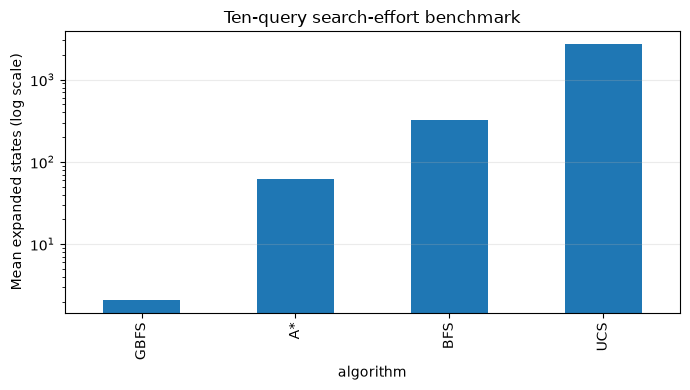
\includegraphics[width=.88\linewidth,height=5cm,keepaspectratio]{labs/visuals/03-notebook-reference.png}
\end{labvisual}
\begin{refoutput}
\begin{lstlisting}[style=utpterminal]
Saved: ['benchmark.csv', 'benchmark_expansions.png', 'benchmark_summary.csv']
Terminal command (from all_experiments):  python -m pytest utils -q
\end{lstlisting}
\end{refoutput}

\textbf{Read the result.} Regenerate this plot rather than copying it. The vertical axis is logarithmic, so the gap between A$^\star$ and UCS is much larger than it looks.
\end{labanswer}

\begin{yourturn}
\begin{enumerate}
  \item \textbf{Add two tests.} Append the two tests below to \texttt{utils/test\_search.py}, then rerun \texttt{python -m pytest utils -q}. The first checks a boundary case for the informed searches. The second pins down what happens when two routes cost the same. Check the result contract, not only the \texttt{found} flag.
  \item \textbf{Use the command line.} Run \texttt{ucs}, \texttt{gbfs} and \texttt{astar} from \texttt{DOH} to \texttt{LIM}. Record cost, route and expansions for each.
  \item \textbf{Find the boundary.} Open \texttt{demo\_robot\_maze.py} and answer: which function plays the role that \texttt{openflights.py} plays for airports, and which lines of \texttt{core.py} had to change for the maze to work?
\end{enumerate}
\begin{lstlisting}[style=utppython]
def test_start_equals_goal_informed():
    h = {"A": 0.0}.get
    for algorithm in (gbfs, astar):
        result = algorithm({"A": []}, "A", "A", h)
        assert result.found and result.path == ["A"]
        assert result.hops == 0 and result.path_cost_km == 0


def test_equal_cost_routes_keep_the_minimum_cost():
    graph = {"S": [("A", 1.0), ("B", 1.0)], "A": [("G", 1.0)], "B": [("G", 1.0)], "G": []}
    assert ucs(graph, "S", "G").path_cost_km == pytest.approx(2.0)
\end{lstlisting}
\end{yourturn}

\begin{expectedfindings}
\begin{enumerate}
  \item \texttt{10 passed}. Question~3's reference output will now read 10 instead of 8, which is correct. If you remove the tests again, it returns to 8.
  \item UCS: 14,856~km via MAD, 3,046 expanded. GBFS: 15,333~km via GRU, 2 expanded. A$^\star$: 14,856~km via MAD, 112 expanded.
  \item \texttt{build\_graph} is the maze's loader, and no line of \texttt{core.py} changed. That is the domain boundary of \figref{fig:domains}: a new domain needs a new loader and nothing else.
\end{enumerate}
\end{expectedfindings}

\begin{troubleshoot}
\begin{description}
  \item[\texttt{No module named pytest}] Your environment is not active, or the requirements were not installed in it. Activate it and run \texttt{pip install -r requirements.txt}.
  \item[\texttt{No module named utils}] Run \texttt{python -m utils} and \texttt{python -m pytest utils} from inside \texttt{all\_experiments/}.
  \item[A test fails after you edited \texttt{core.py}] Good: that is what the tests are for. Read which test failed; each one names one way a search can break.
\end{description}
\end{troubleshoot}

\begin{verification}
\begin{itemize}
  \item All five algorithms return a \texttt{SearchResult} with identical fields.
  \item All tests pass with \texttt{python -m pytest utils -q}, without any dataset.
  \item The command line prints the KUL$\to$HKT$\to$LED$\to$HEL$\to$KEF route and 11,461~km, as Lab~2 found.
  \item Every algorithm succeeds on all ten benchmark queries, and A$^\star$ matches the UCS cost on each.
  \item \texttt{results/lab03/} holds \texttt{benchmark.csv}, \texttt{benchmark\_summary.csv} and \texttt{benchmark\_expansions.png}.
\end{itemize}
\end{verification}

\begin{labdeliverable}
\begin{itemize}
  \item Restart the kernel and run all cells without errors.
  \item Submit the executed notebook, your edited \texttt{test\_search.py} and the generated \texttt{results/lab03/} folder.
  \item Add a short conclusion: recommend a default method for distance-based routing, and explain which module would change for a different graph domain.
\end{itemize}
\end{labdeliverable}
